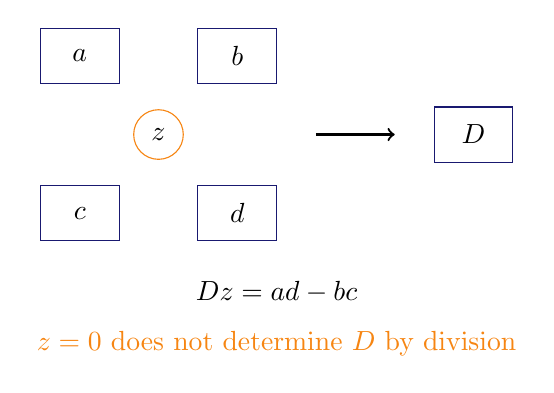
\begin{tikzpicture}[x=1cm,y=1cm]
\foreach \x/\y/\t in {0/1/a,2/1/b,0/-1/c,2/-1/d}{
\node[draw=MidnightBlue,minimum width=1cm,minimum height=.7cm] at (\x,\y) {$\t$};}
\node[draw=BurntOrange,circle,inner sep=4pt] at (1,0) {$z$};
\draw[->,thick] (3,0)--(4,0);
\node[draw=MidnightBlue,minimum width=1cm,minimum height=.7cm] at (5,0) {$D$};
\node at (2.5,-2) {$Dz=ad-bc$};
\node[BurntOrange] at (2.5,-2.65) {$z=0$ does not determine $D$ by division};
\end{tikzpicture}
